% page 10
\frame{
    \frametitle{6.4.2 ガウス過程による回帰}
    出てくる変数:
    \begin{itemize}
        \item $t_n$ :観測変数。$y_n = y(\mathbf{x}_n)$として、
            \begin{gather}
                t_n = y_n + \epsilon_n \tag{6.57}
            \end{gather}
            で定義される。
            まとめて$\bm{\mathsf{t}} = (t_1, \ldots, t_N)^\mathrm{T}$.
        \item $\epsilon_n$ :ノイズ。それぞれの観測値に対して独立に決まる。
           $\beta$をノイズの精度を表す超パラメータとして、
           \begin{gather}
                p(t_n|y_n) = {\cal N} (t_n | y_n, \beta^{-1}) \tag{6.58}
            \end{gather}
            となる。
    \end{itemize}
            
}

% page 11
\frame{
    \frametitle{N個の訓練集合をまとめて書く}
    ノイズは各データ点($y(\mathbf{x}) = $真の値)に対してランダムに決まるので、
    {\optima (6.58)}式をまとめて書くと、
    \begin{gather}
    p(\bm{\mathsf{t}}|\bm{\mathsf{y}})
        = {\cal N} (\bm{\mathsf{t}} | \bm{\mathsf{y}}, 
                \beta^{-1} \mathbf{I}_N).
    \tag{6.59}
    \end{gather}
    となる。ただし、$\mathbf{I}_N$は$N \times N$の単位行列。

    ガウス過程の定義($\mathbb{E}[\bm{\mathsf{y}}] = \mathbf{0}$, 
            $\mathrm{cov}[\bm{\mathsf{y}}] = \mathbf{K}$)より、
    周辺分布$p(\bm{\mathsf{y}})$は、
    \begin{gather}
    p(\bm{\mathsf{y}}) = {\cal N} (\bm{\mathsf{y}} | \mathbf{0}, \mathbf{K}).
        \tag{6.60}
    \end{gather}
    である。

    $\mathbf{K}$を決めるカーネル関数は、二つの点$\mathbf{x}_n$と$\mathbf{x}_m$が
    似ているほど$y(\mathbf{x}_n)$と$y(\mathbf{x}_m)$の相関が高いようなもの
    が選ばれる(たとえばガウスカーネル)。
}

% page 12
\frame{
    \frametitle{データ点のサンプリング}
    \begin{figure}
        \begin{center}
            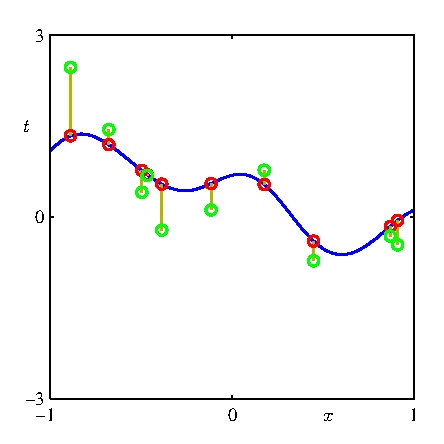
\includegraphics[width=5cm]{charts/Figure6_6.eps}
            \label{6.6}
            \caption{
                \textcolor{blue}{実線}はガウス過程からサンプリングした関数、
                \textcolor{red}{赤い点}
                は入力集合${x_n}$に対応する値$y_n$を表す。\textcolor{green}{緑の丸}
                は、${y_n}$にそれぞれ独立にガウスノイズを加えた点${t_n}$
                を示している。
            }
        \end{center}
    \end{figure}
}

% page 13
\frame{
    \frametitle{観測値の周辺分布}
    $p(\bm{\mathsf{t}} | \bm{\mathsf{y}})$と$p(\bm{\mathsf{y}})$がわかったので、
    次は周辺分布$p(\bm{\mathsf{t}})$を求めたい。すなわち、{\optima (2.115)}式(
    $x$)を用いて、

    \begin{gather}
        p(\bm{\mathsf{t}}) = 
        \int p(\bm{\mathsf{t}} | \bm{\mathsf{y}}) 
            p(\bm{\mathsf{y}}) \d \bm{\mathsf{y}}
        = {\cal N} (\bm{\mathsf{t}} | \mathbf{0}, \mathbf{C}).
        \tag{6.61}
    \end{gather}

    と求まる。共分散行列$\mathbf{C}$の各要素は、
    \begin{gather}
        C(\mathbf{x}_n, \mathbf{x}_m)
        = k(\mathbf{x}_n, \mathbf{x}_m) + \beta^{-1} \gamma_{nm}
        \tag{6.62}
    \end{gather}
    である。$y(\mathbf{x})$と$\epsilon$が互いに独立であるため、共分散もこの二つを
    足し合わせるだけで良い。
}

% page 14
\frame{
    \frametitle{新しい入力を予測する}
    $p(\bm{\mathsf{t}} | \bm{\mathsf{y}})$と$p(\bm{\mathsf{y}})$、
    $p(\bm{\mathsf{y}})$が求まったので、新しい入力ベクトル$\mathbf{x}_{N+1}$
    に対する目標変数$t_{N+1}$を予測したい。そのためには、予測分布
    $p(t_{N+1}|\bm{\mathsf{t}}_N)$を求めなければならない(
    $\bm{\mathsf{t}}_N = (t_1, \ldots, t_N)^{\mathrm{T}}$)。
    
    このとき、
    $p(t_{N+1}|\bm{\mathsf{t}}_N)$は$\bm{\mathsf{t}}_N$だけでなく
    $\mathbf{x}_1, \ldots, \mathbf{x}_N, \mathbf{x}_{N+1}$にも依存しているが、
    簡単のためにそこは省略。\vspace{0.2in}

    {\optima(6.61)}より、$t_1, \ldots, t_{N+1}$の同時分布は、
    \begin{gather}
        p(\bm{\mathsf{t}}_{N+1})
        = {\cal N} (
            \bm{\mathsf{t}}_{N+1} |
            \mathbf{0}, \mathbf{C}_{N+1}
            ).
        \tag{6.64}
    \end{gather}

    このとき、$\mathbf{C}_{N+1}$は、$(N+1) \times (N+1)$の共分散行列で、
    各要素は前頁の{\optima(6.62)}式で与えられる。この式から予測分布を
    求めることができる。
}

% page 15
\frame{
    \frametitle{回帰で求める平均と分散}
    {\optima(6.64)}式の$\mathbf{C}_{N+1}$を分割して、
    \begin{gather}
        \mathbf{C}_{N+1} = 
        \begin{pmatrix}
            \mathbf{C}_N & \mathbf{k} \\
            \mathbf{k}^{\mathrm{T}} & c
        \end{pmatrix}
        \tag{6.65}
    \end{gather}
    とする。$\mathbf{k}$は、要素
    $k(\mathbf{x}_n, \mathbf{x}_{N+1} (n = 1, \ldots, N)$を持つ
    ベクトルであり、$c = k(\mathbf{x}_{N+1}, \mathbf{x}_{N+1}) + \beta^{-1}$
    とする。\vspace{0.2in}

    いろいろ計算すると、$p(t_{N+1} | \bm{\mathsf{t}})$は、以下のような平均と
    共分散を持つガウス分布であることがわかる。
    \begin{align}
        m(\mathbf{x}_{N+1}) 
            &= \mathbf{k}^\mathrm{T} \mathbf{C}_{N}^{-1} \bm{\mathsf{t}}
            \tag{6.66} \\
        \sigma^2 (\mathbf{x}_{N+1}) 
            &= c - \mathbf{k}^\mathrm{T} \mathbf{C}_N^{-1} \mathbf{k}
            \tag{6.67}
    \end{align}
}

% page 16
\frame{
    \frametitle{ガウス過程による回帰:例}

    \begin{figure}
        \begin{center}
            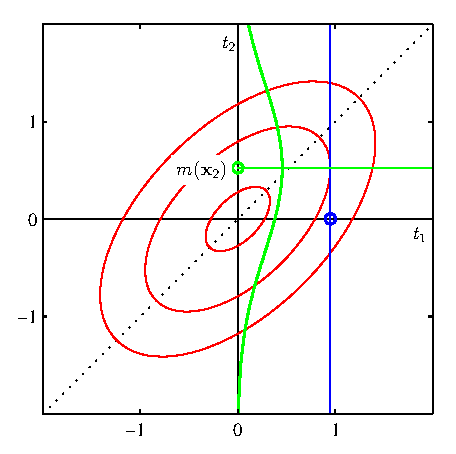
\includegraphics[width=5cm]{charts/Figure6_7.eps}
            \label{6.7}
            \caption{
                訓練データとテストデータが1つずつの場合のガウス過程
                による回帰のしくみ。\textcolor{red}{赤色の楕円}が、
                同時分布$p(t_1, t_2)$の 等高線を示している。$t_1$は
                訓練データ(\textcolor{blue}{青い点})。
                \textcolor{green}{緑色の線}は$p(t_2|t_1)$。
                楕円を青いところで切るとこんな感じになる。
            }
        \end{center}
    \end{figure}
}

% page 17
\frame{
    \frametitle{ガウス過程の適用例}
    \begin{figure}
        \begin{center}
            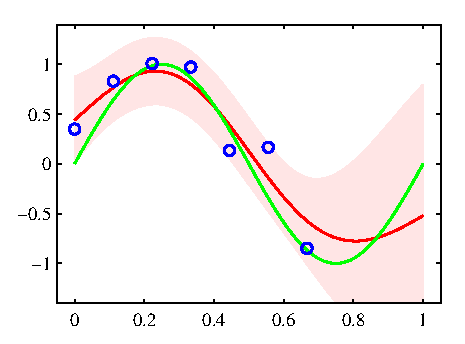
\includegraphics[width=4cm]{charts/Figure6_8.eps}
            \caption{
                \textcolor{red}{赤い線}は正弦関数を表している。
                \textcolor{blue}{青い点}はそこからガウス分布に従う
                ノイズを加えてサンプリングされたデータ点。
                \textcolor{green}{緑色の実線}がガウス過程による平均、
                \textcolor{red}{ピンク色の領域}がガウス過程による分散
                (標準偏差の2倍)を表している。データが疎な部分(右端付近)
                では不確かさ(分散)が大きくなっているのがわかる。
            }
        \end{center}
    \end{figure}
}

% page 18
\frame{
    \frametitle{よく使われるカーネル}
    ガウス過程回帰に使われるカーネル関数として、以下のようなものがある。

    4つの超パラメータ($\theta_0, \theta_1, \theta_2, \theta_3$)をもつ。
    \begin{gather}
        k(\mathbf{x}_n, \mathbf{x}_m)
        = \theta_0 \exp \left\{
            - \frac{\theta_1}{2} \| \mathbf{x}_n - \mathbf{x}_m \|^2
        \right\}
        + \theta_2
        + \theta_3 \mathbf{x}_n^{\mathrm{T}} \mathbf{x}_m.
        \tag{6.63}
    \end{gather}

    \begin{figure}
        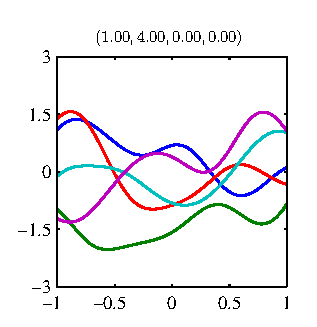
\includegraphics[width=2cm]{charts/Figure6_5a.eps}
        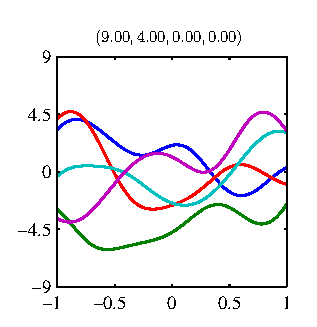
\includegraphics[width=2cm]{charts/Figure6_5b.eps}
        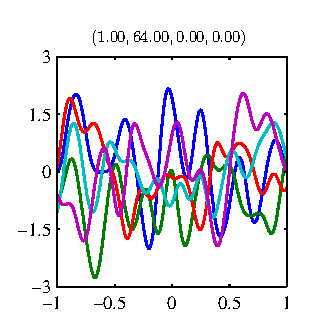
\includegraphics[width=2cm]{charts/Figure6_5c.eps}

        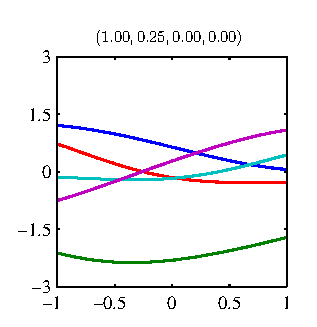
\includegraphics[width=2cm]{charts/Figure6_5d.eps}
        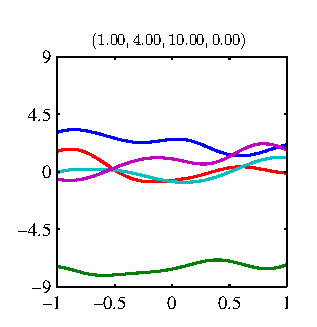
\includegraphics[width=2cm]{charts/Figure6_5e.eps}
        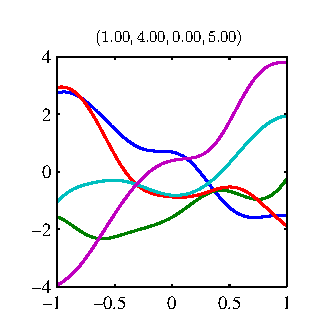
\includegraphics[width=2cm]{charts/Figure6_5f.eps}
    \end{figure}
}

% page 19
\frame{
    \frametitle{制約など}
    カーネル関数は何でも良いが、{\optima(6.62)}で与えられる共分散行列が
    正定値でなければならない。\vspace{0.2in}

    また、予測分布の平均{\optima(6.66)}は、$\mathbf{x}_{N+1}$の関数として
    \begin{gather}
        m(\mathbf{x}_{N+1}) = \sum_{n=1}^N a_n k(\mathbf{x}_n, \mathbf{x}_{N+1})
        \tag{6.68}
    \end{gather}
    と表すことができる。ただし、$a_n$は$\mathbf{C}_N^{-1} \bm{\mathsf{t}}$の
    $n$番目の要素。この式を用いると、$\mathbf{K}$($N \times N$次元)の代わりに
    $M$個の基底関数で表すことができ、$M \times M$の行列の逆行列を求めればすむ。
    
    このため、データ数$N$に比べてモデル数$M$が少ないような場合は、計算量を減らす
    ことができる。ただし、カーネル関数の中には無限個の基底関数でしか表せないものが
    あり、そうしたものにはこの方法は使えない。
}

% page 20
\frame{
    \frametitle{6.4.2 まとめ}
    \begin{itemize}
        \item ノイズ$\epsilon_n$を加えた観測値$\bm{\mathsf{t}}$
            から、新たなデータに対する予測分布$p(t_{N+1}|\bm{\mathsf{t}})$
            を求めることができた。
        \item 予測分布は、
            \begin{align}
        m(\mathbf{x}_{N+1}) 
            &= \mathbf{k}^\mathrm{T} \mathbf{C}_{N}^{-1} \bm{\mathsf{t}}
            \tag{6.66} \\
        \sigma^2 (\mathbf{x}_{N+1}) 
            &= c - \mathbf{k}^\mathrm{T} \mathbf{C}_N^{-1} \mathbf{k}
            \tag{6.67}
    \end{align}
    という平均と共分散を持つガウス分布になる。
\item $N \times N$の共分散行列の逆行列$\mathbf{C}_N^{-1}$を求めなければならないので、
    計算時間は$O(N^3)$となってしまう。基底関数を用いて$\mathbf{S}_N$の逆行列を求めれば
    (カーネルトリックは使えないが)計算量は$O(M^3)$になる。

    \end{itemize}
}
